\documentclass{standalone}
\usepackage{tikz}
\usetikzlibrary{patterns, positioning}


\begin{document}
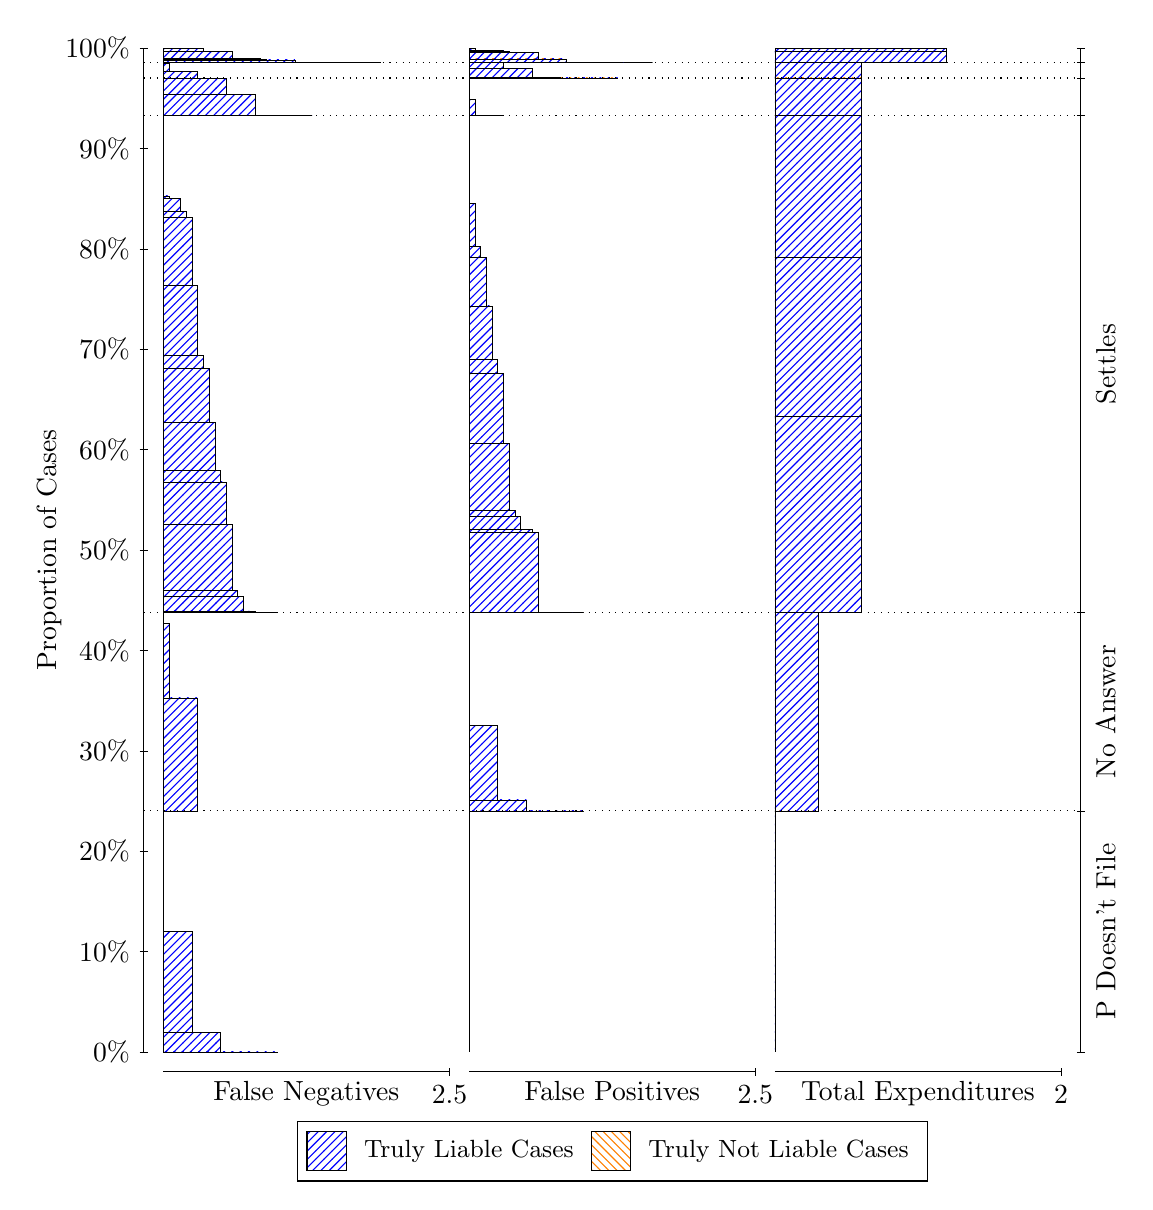
\begin{tikzpicture}
\draw[black, very thin] (1.5,1.75) -- (1.5,14.5);
\node[rotate=90, text=black, anchor=center] at (0.3, 8.125) {Proportion of Cases};
\draw[black, very thin] (1.45,1.75) -- (1.55,1.75);
\node[text=black, anchor=east] at (1.45, 1.75) {0\%};
\draw[black, very thin] (1.45,3.025) -- (1.55,3.025);
\node[text=black, anchor=east] at (1.45, 3.025) {10\%};
\draw[black, very thin] (1.45,4.3) -- (1.55,4.3);
\node[text=black, anchor=east] at (1.45, 4.3) {20\%};
\draw[black, very thin] (1.45,5.575) -- (1.55,5.575);
\node[text=black, anchor=east] at (1.45, 5.575) {30\%};
\draw[black, very thin] (1.45,6.85) -- (1.55,6.85);
\node[text=black, anchor=east] at (1.45, 6.85) {40\%};
\draw[black, very thin] (1.45,8.125) -- (1.55,8.125);
\node[text=black, anchor=east] at (1.45, 8.125) {50\%};
\draw[black, very thin] (1.45,9.4) -- (1.55,9.4);
\node[text=black, anchor=east] at (1.45, 9.4) {60\%};
\draw[black, very thin] (1.45,10.675) -- (1.55,10.675);
\node[text=black, anchor=east] at (1.45, 10.675) {70\%};
\draw[black, very thin] (1.45,11.95) -- (1.55,11.95);
\node[text=black, anchor=east] at (1.45, 11.95) {80\%};
\draw[black, very thin] (1.45,13.225) -- (1.55,13.225);
\node[text=black, anchor=east] at (1.45, 13.225) {90\%};
\draw[black, very thin] (1.45,14.5) -- (1.55,14.5);
\node[text=black, anchor=east] at (1.45, 14.5) {100\%};

\draw[black, very thin] (13.4,1.75) -- (13.4,14.5);
\draw[black, very thin] (13.35,1.75) -- (13.45,1.75);
\node[anchor=west] at (13.35, 1.75) {};
\draw[black, very thin] (13.35,4.8113) -- (13.45,4.8113);
\node[anchor=west] at (13.35, 4.8113) {};
\draw[black, very thin] (13.35,7.3329) -- (13.45,7.3329);
\node[anchor=west] at (13.35, 7.3329) {};
\draw[black, very thin] (13.35,13.641) -- (13.45,13.641);
\node[anchor=west] at (13.35, 13.641) {};
\draw[black, very thin] (13.35,14.12) -- (13.45,14.12);
\node[anchor=west] at (13.35, 14.12) {};
\draw[black, very thin] (13.35,14.318) -- (13.45,14.318);
\node[anchor=west] at (13.35, 14.318) {};
\draw[black, very thin] (13.35,14.5) -- (13.45,14.5);
\node[anchor=west] at (13.35, 14.5) {};

\draw[black, very thin, pattern color=blue, pattern=north east lines] (1.75,1.75) rectangle (3.2033,1.75);
\draw[black, very thin, pattern color=blue, pattern=north east lines] (1.75,1.75) rectangle (2.84,1.7524);
\draw[black, very thin, pattern color=blue, pattern=north east lines] (1.75,1.7524) rectangle (2.4767,1.9965);
\draw[black, very thin, pattern color=blue, pattern=north east lines] (1.75,1.9965) rectangle (2.1133,3.2837);
\draw[black, very thin, pattern color=orange, pattern=north west lines] (1.75,3.2837) rectangle (1.75,3.2837);
\draw[black, very thin, pattern color=blue, pattern=north east lines] (1.75,3.2837) rectangle (1.75,4.8113);
\draw[black, very thin, pattern color=blue, pattern=north east lines] (1.75,4.8113) rectangle (2.186,6.2462);
\draw[black, very thin, pattern color=blue, pattern=north east lines] (1.75,6.2462) rectangle (1.8227,7.1935);
\draw[black, very thin, pattern color=orange, pattern=north west lines] (1.75,7.1935) rectangle (1.75,7.1935);
\draw[black, very thin, pattern color=blue, pattern=north east lines] (1.75,7.1935) rectangle (1.75,7.3329);
\draw[black, very thin, pattern color=blue, pattern=north east lines] (1.75,7.3329) rectangle (3.2033,7.3329);
\draw[black, very thin, pattern color=blue, pattern=north east lines] (1.75,7.3329) rectangle (3.058,7.3331);
\draw[black, very thin, pattern color=blue, pattern=north east lines] (1.75,7.3331) rectangle (2.9127,7.3499);
\draw[black, very thin, pattern color=blue, pattern=north east lines] (1.75,7.3499) rectangle (2.84,7.3504);
\draw[black, very thin, pattern color=blue, pattern=north east lines] (1.75,7.3504) rectangle (2.7673,7.5312);
\draw[black, very thin, pattern color=blue, pattern=north east lines] (1.75,7.5312) rectangle (2.6947,7.6122);
\draw[black, very thin, pattern color=blue, pattern=north east lines] (1.75,7.6122) rectangle (2.622,8.4488);
\draw[black, very thin, pattern color=blue, pattern=north east lines] (1.75,8.4488) rectangle (2.5493,8.9891);
\draw[black, very thin, pattern color=blue, pattern=north east lines] (1.75,8.9891) rectangle (2.4767,9.1312);
\draw[black, very thin, pattern color=blue, pattern=north east lines] (1.75,9.1312) rectangle (2.404,9.7498);
\draw[black, very thin, pattern color=blue, pattern=north east lines] (1.75,9.7498) rectangle (2.3313,10.432);
\draw[black, very thin, pattern color=blue, pattern=north east lines] (1.75,10.432) rectangle (2.2587,10.599);
\draw[black, very thin, pattern color=blue, pattern=north east lines] (1.75,10.599) rectangle (2.186,11.49);
\draw[black, very thin, pattern color=blue, pattern=north east lines] (1.75,11.49) rectangle (2.1133,12.348);
\draw[black, very thin, pattern color=blue, pattern=north east lines] (1.75,12.348) rectangle (2.0407,12.424);
\draw[black, very thin, pattern color=blue, pattern=north east lines] (1.75,12.424) rectangle (1.968,12.587);
\draw[black, very thin, pattern color=blue, pattern=north east lines] (1.75,12.587) rectangle (1.8953,12.589);
\draw[black, very thin, pattern color=blue, pattern=north east lines] (1.75,12.589) rectangle (1.8227,12.621);
\draw[black, very thin, pattern color=orange, pattern=north west lines] (1.75,12.621) rectangle (1.75,12.621);
\draw[black, very thin, pattern color=blue, pattern=north east lines] (1.75,12.621) rectangle (1.75,13.641);
\draw[black, very thin, pattern color=blue, pattern=north east lines] (1.75,13.641) rectangle (3.6393,13.641);
\draw[black, very thin, pattern color=blue, pattern=north east lines] (1.75,13.641) rectangle (3.276,13.646);
\draw[black, very thin, pattern color=blue, pattern=north east lines] (1.75,13.646) rectangle (2.9127,13.911);
\draw[black, very thin, pattern color=blue, pattern=north east lines] (1.75,13.911) rectangle (2.5493,14.118);
\draw[black, very thin, pattern color=blue, pattern=north east lines] (1.75,14.118) rectangle (2.186,14.12);
\draw[black, very thin, pattern color=orange, pattern=north west lines] (1.75,14.12) rectangle (1.75,14.12);
\draw[black, very thin, pattern color=blue, pattern=north east lines] (1.75,14.12) rectangle (2.186,14.199);
\draw[black, very thin, pattern color=blue, pattern=north east lines] (1.75,14.199) rectangle (1.8227,14.31);
\draw[black, very thin, pattern color=orange, pattern=north west lines] (1.75,14.31) rectangle (1.75,14.31);
\draw[black, very thin, pattern color=blue, pattern=north east lines] (1.75,14.31) rectangle (1.75,14.318);
\draw[black, very thin, pattern color=blue, pattern=north east lines] (1.75,14.318) rectangle (4.5113,14.318);
\draw[black, very thin, pattern color=blue, pattern=north east lines] (1.75,14.318) rectangle (4.148,14.318);
\draw[black, very thin, pattern color=blue, pattern=north east lines] (1.75,14.318) rectangle (3.7847,14.322);
\draw[black, very thin, pattern color=blue, pattern=north east lines] (1.75,14.322) rectangle (3.712,14.322);
\draw[black, very thin, pattern color=blue, pattern=north east lines] (1.75,14.322) rectangle (3.4213,14.348);
\draw[black, very thin, pattern color=blue, pattern=north east lines] (1.75,14.348) rectangle (3.3487,14.348);
\draw[black, very thin, pattern color=blue, pattern=north east lines] (1.75,14.348) rectangle (3.058,14.355);
\draw[black, very thin, pattern color=blue, pattern=north east lines] (1.75,14.355) rectangle (2.9853,14.371);
\draw[black, very thin, pattern color=blue, pattern=north east lines] (1.75,14.371) rectangle (2.6947,14.371);
\draw[black, very thin, pattern color=blue, pattern=north east lines] (1.75,14.371) rectangle (2.622,14.456);
\draw[black, very thin, pattern color=blue, pattern=north east lines] (1.75,14.456) rectangle (2.3313,14.456);
\draw[black, very thin, pattern color=blue, pattern=north east lines] (1.75,14.456) rectangle (2.2587,14.498);
\draw[black, very thin, pattern color=blue, pattern=north east lines] (1.75,14.498) rectangle (1.8953,14.5);
\draw[black, very thin, pattern color=orange, pattern=north west lines] (1.75,14.5) rectangle (1.75,14.5);
\draw[black, very thin, pattern color=blue, pattern=north east lines] (1.75,14.5) rectangle (1.75,14.5);
\draw[black, very thin, pattern color=orange, pattern=north west lines] (5.6333,1.75) rectangle (5.6333,1.75);
\draw[black, very thin, pattern color=blue, pattern=north east lines] (5.6333,1.75) rectangle (5.6333,4.8113);
\draw[black, very thin, pattern color=orange, pattern=north west lines] (5.6333,4.8113) rectangle (7.0867,4.8113);
\draw[black, very thin, pattern color=blue, pattern=north east lines] (5.6333,4.8113) rectangle (7.0867,4.8113);
\draw[black, very thin, pattern color=blue, pattern=north east lines] (5.6333,4.8113) rectangle (6.7233,4.8115);
\draw[black, very thin, pattern color=blue, pattern=north east lines] (5.6333,4.8115) rectangle (6.36,4.9507);
\draw[black, very thin, pattern color=blue, pattern=north east lines] (5.6333,4.9507) rectangle (5.9967,5.898);
\draw[black, very thin, pattern color=blue, pattern=north east lines] (5.6333,5.898) rectangle (5.6333,7.3329);
\draw[black, very thin, pattern color=orange, pattern=north west lines] (5.6333,7.3329) rectangle (7.0867,7.3329);
\draw[black, very thin, pattern color=blue, pattern=north east lines] (5.6333,7.3329) rectangle (7.0867,7.3329);
\draw[black, very thin, pattern color=orange, pattern=north west lines] (5.6333,7.3329) rectangle (6.9413,7.3329);
\draw[black, very thin, pattern color=blue, pattern=north east lines] (5.6333,7.3329) rectangle (6.9413,7.3329);
\draw[black, very thin, pattern color=orange, pattern=north west lines] (5.6333,7.3329) rectangle (6.796,7.3329);
\draw[black, very thin, pattern color=blue, pattern=north east lines] (5.6333,7.3329) rectangle (6.796,7.3329);
\draw[black, very thin, pattern color=blue, pattern=north east lines] (5.6333,7.3329) rectangle (6.7233,7.3329);
\draw[black, very thin, pattern color=orange, pattern=north west lines] (5.6333,7.3329) rectangle (6.6507,7.3329);
\draw[black, very thin, pattern color=blue, pattern=north east lines] (5.6333,7.3329) rectangle (6.6507,7.3345);
\draw[black, very thin, pattern color=blue, pattern=north east lines] (5.6333,7.3345) rectangle (6.578,7.3347);
\draw[black, very thin, pattern color=orange, pattern=north west lines] (5.6333,7.3347) rectangle (6.5053,7.3347);
\draw[black, very thin, pattern color=blue, pattern=north east lines] (5.6333,7.3347) rectangle (6.5053,8.353);
\draw[black, very thin, pattern color=blue, pattern=north east lines] (5.6333,8.353) rectangle (6.4327,8.3849);
\draw[black, very thin, pattern color=blue, pattern=north east lines] (5.6333,8.3849) rectangle (6.36,8.3865);
\draw[black, very thin, pattern color=blue, pattern=north east lines] (5.6333,8.3865) rectangle (6.2873,8.5492);
\draw[black, very thin, pattern color=blue, pattern=north east lines] (5.6333,8.5492) rectangle (6.2147,8.6257);
\draw[black, very thin, pattern color=blue, pattern=north east lines] (5.6333,8.6257) rectangle (6.142,9.4834);
\draw[black, very thin, pattern color=blue, pattern=north east lines] (5.6333,9.4834) rectangle (6.0693,10.374);
\draw[black, very thin, pattern color=blue, pattern=north east lines] (5.6333,10.374) rectangle (5.9967,10.541);
\draw[black, very thin, pattern color=blue, pattern=north east lines] (5.6333,10.541) rectangle (5.924,11.224);
\draw[black, very thin, pattern color=blue, pattern=north east lines] (5.6333,11.224) rectangle (5.8513,11.842);
\draw[black, very thin, pattern color=blue, pattern=north east lines] (5.6333,11.842) rectangle (5.7787,11.985);
\draw[black, very thin, pattern color=blue, pattern=north east lines] (5.6333,11.985) rectangle (5.706,12.525);
\draw[black, very thin, pattern color=blue, pattern=north east lines] (5.6333,12.525) rectangle (5.6333,13.641);
\draw[black, very thin, pattern color=orange, pattern=north west lines] (5.6333,13.641) rectangle (6.0693,13.641);
\draw[black, very thin, pattern color=blue, pattern=north east lines] (5.6333,13.641) rectangle (6.0693,13.643);
\draw[black, very thin, pattern color=blue, pattern=north east lines] (5.6333,13.643) rectangle (5.706,13.85);
\draw[black, very thin, pattern color=blue, pattern=north east lines] (5.6333,13.85) rectangle (5.6333,14.12);
\draw[black, very thin, pattern color=orange, pattern=north west lines] (5.6333,14.12) rectangle (7.5227,14.12);
\draw[black, very thin, pattern color=blue, pattern=north east lines] (5.6333,14.12) rectangle (7.5227,14.12);
\draw[black, very thin, pattern color=blue, pattern=north east lines] (5.6333,14.12) rectangle (7.1593,14.12);
\draw[black, very thin, pattern color=blue, pattern=north east lines] (5.6333,14.12) rectangle (6.796,14.129);
\draw[black, very thin, pattern color=blue, pattern=north east lines] (5.6333,14.129) rectangle (6.4327,14.24);
\draw[black, very thin, pattern color=blue, pattern=north east lines] (5.6333,14.24) rectangle (6.0693,14.318);
\draw[black, very thin, pattern color=orange, pattern=north west lines] (5.6333,14.318) rectangle (7.9587,14.318);
\draw[black, very thin, pattern color=blue, pattern=north east lines] (5.6333,14.318) rectangle (7.9587,14.318);
\draw[black, very thin, pattern color=orange, pattern=north west lines] (5.6333,14.318) rectangle (7.5953,14.318);
\draw[black, very thin, pattern color=blue, pattern=north east lines] (5.6333,14.318) rectangle (7.5953,14.318);
\draw[black, very thin, pattern color=orange, pattern=north west lines] (5.6333,14.318) rectangle (7.232,14.318);
\draw[black, very thin, pattern color=blue, pattern=north east lines] (5.6333,14.318) rectangle (7.232,14.32);
\draw[black, very thin, pattern color=blue, pattern=north east lines] (5.6333,14.32) rectangle (6.8687,14.362);
\draw[black, very thin, pattern color=orange, pattern=north west lines] (5.6333,14.362) rectangle (6.8687,14.362);
\draw[black, very thin, pattern color=blue, pattern=north east lines] (5.6333,14.362) rectangle (6.8687,14.362);
\draw[black, very thin, pattern color=orange, pattern=north west lines] (5.6333,14.362) rectangle (6.796,14.362);
\draw[black, very thin, pattern color=blue, pattern=north east lines] (5.6333,14.362) rectangle (6.796,14.362);
\draw[black, very thin, pattern color=blue, pattern=north east lines] (5.6333,14.362) rectangle (6.5053,14.446);
\draw[black, very thin, pattern color=blue, pattern=north east lines] (5.6333,14.446) rectangle (6.5053,14.447);
\draw[black, very thin, pattern color=orange, pattern=north west lines] (5.6333,14.447) rectangle (6.4327,14.447);
\draw[black, very thin, pattern color=blue, pattern=north east lines] (5.6333,14.447) rectangle (6.4327,14.447);
\draw[black, very thin, pattern color=blue, pattern=north east lines] (5.6333,14.447) rectangle (6.142,14.455);
\draw[black, very thin, pattern color=blue, pattern=north east lines] (5.6333,14.455) rectangle (6.142,14.463);
\draw[black, very thin, pattern color=blue, pattern=north east lines] (5.6333,14.463) rectangle (6.0693,14.47);
\draw[black, very thin, pattern color=orange, pattern=north west lines] (5.6333,14.47) rectangle (6.0693,14.47);
\draw[black, very thin, pattern color=blue, pattern=north east lines] (5.6333,14.47) rectangle (6.0693,14.47);
\draw[black, very thin, pattern color=blue, pattern=north east lines] (5.6333,14.47) rectangle (5.7787,14.47);
\draw[black, very thin, pattern color=blue, pattern=north east lines] (5.6333,14.47) rectangle (5.7787,14.47);
\draw[black, very thin, pattern color=blue, pattern=north east lines] (5.6333,14.47) rectangle (5.706,14.495);
\draw[black, very thin, pattern color=blue, pattern=north east lines] (5.6333,14.495) rectangle (5.706,14.496);
\draw[black, very thin, pattern color=blue, pattern=north east lines] (5.6333,14.496) rectangle (5.6333,14.5);
\draw[black, very thin, pattern color=orange, pattern=north west lines] (9.5167,1.75) rectangle (9.5167,1.75);
\draw[black, very thin, pattern color=blue, pattern=north east lines] (9.5167,1.75) rectangle (9.5167,4.8113);
\draw[black, very thin, pattern color=orange, pattern=north west lines] (9.5167,4.8113) rectangle (10.062,4.8113);
\draw[black, very thin, pattern color=blue, pattern=north east lines] (9.5167,4.8113) rectangle (10.062,7.3329);
\draw[black, very thin, pattern color=orange, pattern=north west lines] (9.5167,7.3329) rectangle (10.607,7.3329);
\draw[black, very thin, pattern color=blue, pattern=north east lines] (9.5167,7.3329) rectangle (10.607,9.8181);
\draw[black, very thin, pattern color=orange, pattern=north west lines] (9.5167,9.8181) rectangle (10.607,9.8181);
\draw[black, very thin, pattern color=blue, pattern=north east lines] (9.5167,9.8181) rectangle (10.607,11.837);
\draw[black, very thin, pattern color=orange, pattern=north west lines] (9.5167,11.837) rectangle (10.607,11.837);
\draw[black, very thin, pattern color=blue, pattern=north east lines] (9.5167,11.837) rectangle (10.607,13.641);
\draw[black, very thin, pattern color=orange, pattern=north west lines] (9.5167,13.641) rectangle (10.607,13.641);
\draw[black, very thin, pattern color=blue, pattern=north east lines] (9.5167,13.641) rectangle (10.607,14.12);
\draw[black, very thin, pattern color=orange, pattern=north west lines] (9.5167,14.12) rectangle (10.607,14.12);
\draw[black, very thin, pattern color=blue, pattern=north east lines] (9.5167,14.12) rectangle (10.607,14.318);
\draw[black, very thin, pattern color=orange, pattern=north west lines] (9.5167,14.318) rectangle (11.697,14.318);
\draw[black, very thin, pattern color=blue, pattern=north east lines] (9.5167,14.318) rectangle (11.697,14.454);
\draw[black, very thin, pattern color=orange, pattern=north west lines] (9.5167,14.454) rectangle (11.697,14.454);
\draw[black, very thin, pattern color=blue, pattern=north east lines] (9.5167,14.454) rectangle (11.697,14.5);
\draw[black, dotted] (1.5,4.8113) -- (13.4,4.8113);
\draw[black, dotted] (1.5,7.3329) -- (13.4,7.3329);
\draw[black, dotted] (1.5,13.641) -- (13.4,13.641);
\draw[black, dotted] (1.5,14.12) -- (13.4,14.12);
\draw[black, dotted] (1.5,14.318) -- (13.4,14.318);
\draw[black, very thin] (1.75,1.5) -- (5.3833,1.5);
\node[text=black, anchor=north] at (3.5667, 1.5) {False Negatives};
\draw[black, very thin] (5.3833,1.45) -- (5.3833,1.55);
\node[text=black, anchor=north] at (5.3833, 1.45) {2.5};

\draw[black, very thin] (5.6333,1.5) -- (9.2667,1.5);
\node[text=black, anchor=north] at (7.45, 1.5) {False Positives};
\draw[black, very thin] (9.2667,1.45) -- (9.2667,1.55);
\node[text=black, anchor=north] at (9.2667, 1.45) {2.5};

\draw[black, very thin] (9.5167,1.5) -- (13.15,1.5);
\node[text=black, anchor=north] at (11.333, 1.5) {Total Expenditures};
\draw[black, very thin] (13.15,1.45) -- (13.15,1.55);
\node[text=black, anchor=north] at (13.15, 1.45) {2};

\node[text=black, centered, rotate=90] at (13.72, 3.2806) {P Doesn't File};
\node[text=black, centered, rotate=90] at (13.72, 6.0721) {No Answer};
\node[text=black, centered, rotate=90] at (13.72, 10.487) {Settles};




\draw (7.449999999999999,1.5) node[draw=none] (baseCoordinate) {};
\begin{scope}[align=center]
        \matrix[scale=0.5, draw=black, below=0.5cm of baseCoordinate, nodes={draw}, column sep=0.1cm]{
            \node[rectangle, draw, minimum width=0.5cm, minimum height=0.5cm, pattern color=blue, pattern=north east lines] {}; &
            \node[draw=none, font=\small, text=black] (B) {Truly Liable Cases}; &
            \node[rectangle, draw, minimum width=0.5cm, minimum height=0.5cm, pattern color=orange, pattern=north west lines] {}; &
            \node[draw=none, font=\small, text=black] (B) {Truly Not Liable Cases}; \\
            };
\end{scope}

\end{tikzpicture}
\end{document}